\documentclass[12pt,letterpaper]{article}

\usepackage{pslatex}
\usepackage{apacite}
\usepackage{url}
\usepackage{graphicx}
\usepackage{todonotes}

\renewcommand\bibliographytypesize{\small}

\title{Emergent Collective Sensing \\in Human Groups}

\author{
RH or PK --- to be randomized \thanks{MIT Computer Science and Artificial Intelligence Laboratory}
\vspace{-.5em}
\and 
PK or RH --- to be randomized \thanks{Stanford Department of Psychology}
\vspace{-.5em}
\and 
Hongbo Fang (hongbofa@andrew.cmu.edu)\thanks{Department of Computer Science, Carnegie Mellon University}
\vspace{-.5em}
\and
Alex ``Sandy'' Pentland (pentland@mit.edu)\thanks{MIT Media Lab}
\and 
Noah D. Goodman (ngoodman@stanford.edu)$^\dagger$
\and 
Joshua B. Tenenbaum (jbt@mit.edu)$^*$
}

\date{}
\begin{document}

\maketitle
\vspace{-2em}

\begin{abstract}

Groups of agents are capable of solving problems that no individual can solve in isolation. 
While intelligent behavior emerges only at large group sizes for many nonhuman species (e.g. fish or insects), humans rapidly benefit from social interaction even in small teams. 
In this paper, we take a comparative approach to identity candidate  mechanisms of social cognition that may account for distinctively human forms of collective intelligence. 
%While a variety of simple mechanisms have been proposed to account for 
%Despite its importance, human collective intelligence remains enigmatic.  
%We know what features are predictive of collective intelligence in human groups, but we do not understand the specific mechanisms that lead to the emergence of this distributed information processing ability. 
%In contrast, there is a well-developed literature of experiments that have exposed the mechanisms of collective intelligence in nonhuman animal species.
In Experiment 1, we designed a collective search paradigm inspired by the nonhuman animal literature and found that performance quickly improves as a function of group size for groups of up to six human participants.
%in order to better understand the mechanisms that may underlie the emergence of collective intelligence in human groups.  
In Experiment 2, we placed human participants in scenarios with artificial agents that were constructed to expose the role of two candidate mechanisms: independent exploration and targeted copying based on social inferences about who is currently successful. 
%We further validated our experimental results by implementing these mechanisms in a computational model: a simulated agent equipped with these mechanisms explained human performance better than models relying on other simple heuristics that have been proposed for nonhuman animals.
Finally, in Experiment 3, we generalize our results to a more complex and noisy environment. 
In sum, even the most rudimentary mechanisms of human social cognition may allow us to derive the benefits of collective intelligence in smaller groups and over shorter timescales than nonhuman animals.

\textbf{Keywords:}
  collective intelligence; distributed cognition;
  social cognition; social computation; online experiments
\end{abstract}

\section{Introduction}

% Paragraph 1: set up the idea of collective intelligence (i.e. motivating why people would care about the secondary question of the individual cognitive mechanisms undelrying it) and then pose the problem of what makes human CI different) i.e. point out that there seems to be not just differences in the scale of these successes (e.g. cumulative human culture) but also the group sizes and timescales at which benefits begin to emerge, so there may be different processes at play. then pose question about what allows this uniquely human style of collective intelligence to get off the ground.
From ant colonies to basketball teams, groups of agents are able to accomplish feats of intelligence beyond the reach of any individual.
Groups are not only able to distribute complex computations across agents more efficiently (cite?), but also gain access to new emergent mechanisms. 
When agents can observe and learn from one another, solutions can be transmitted; agents no longer need to independently obtain all of their information from direct experience with the world.
While collective intelligence is ubiquitous across different species, however, the successes of human culture appear to be distinctive in several ways, suggesting that human collective intelligence may depend on fundamentally different mechanisms \cite{tomasello_natural_2014, henrich2017secret, laland2017darwin}.
Here we explore the idea that one clue to these mechanisms may be found in the \emph{group size} at which the benefits of collective intelligence begin to emerge.

While much work in social learning has focused on what rules or heuristic mechanisms underlie collective intelligence, cognitive scientists have shifted the questions towards what cognitive abilities are needed to deploy the rules that do yield collective intelligence.  Some heuristics involve metacognitive analysis, such as copy-when-uncertain. Other heuristic involve social reasoning, such as copy-the-most-successful or prestige bias.  In the present work we connect this literature on heuristics for social learning and cumulative cultural evolution, which often focus on swarm-like or "mean-field" collective intelligence of very large groups, which have focused less on cognitive abilities, with the key collective intelligence literature from organization science focused on factors explaining collective intelligence in small groups, which have focused more on cognitive abilities.

Researchers in organization science have identified the metacognitive agent reasoning abilities, in particular theory of mind, as a key predictive factor of collective intelligence in small groups performing collaborative work.  Here, we ask how agent reasoning abilities are important to heuristic social learning mechanisms of collective intelligence.  With an eye towards comparing human collective intelligence to non-human animal collective intelligence, we seek to answer this question in the context of an empirical domain where as near as possible direct comparison is rendered feasible.  Most empirical work mechanisms of social learning for collective intelligence in non-human animal species has been conducted with fish and social insects.

%A distinctive component of human civilization compared to the rest of the animal kingdom is that we have a human civilization at all. This observation has motivated a great deal of work in the fields of collective intelligence, social learning, and evolutionary biology. What makes human collective intelligence distinct compared to the collective intelligence displayed by other animal species?



%There are of course many ways in which human reasoning and especially human social cognition are distinctive as compared to the expression of similar abilities observed in other animals.  People engage in extraordinarily complex forms of tool use, language use, and both explicit and intuitive pedagogy.

%A variety of forms of social cognition have been documented in many species, such as social interactions in primates, theory of mind in crows, or teaching of tool use in dolphins, but much of the work on these advanced forms of social cognition in non-human animals focuses on interacting pairs. With a few exceptions like roving bands of apes, work on collective intelligence in non-human animals has focused on large groups and swarm intelligence such as in social insects and fish. These swarm intelligence contexts, such as searching for home or food or evading predators, afford simplistic heuristic models of collective intelligence to describe the success of the collective behavior of these species.

%Heyes recently proposed that people may still be distinctive even in these kinds of simpler swarm-like social learning contexts, arguing that people by knowing who to know create distinctive forms of social learning.  This theory echos a variety of results on collective intelligence from organization science, including on transactive memory, the importance of theory of mind in small-group collaboration, and laboratory studies showing the adaptivity of dynamic social networks.

Here, we aim to establish this claim through an experimental paradigm that mirrors the type of environment in which a particular species of fish have demonstrated collective intelligence. By situating people in this fish-like collective intelligence task, we can more directly as: What makes people different from fish in this context?







In the present paper we harness recent technical advances in running
real-time, networked experiments on the web
\cite{hawkins_conducting_2014} to develop and test a model of
collective human behavior.  We build on a recent experiment designed
to study the collective behavior of a particular species of fish
\cite{berdahl_emergent_2013} that is one of the clearest illustrations
of collective intelligence in a nonhuman animal group.  In this
previous experiment, the researchers studied a type of fish called the
golden shiner that prefers to spend time in dark areas of the water,
presumably to avoid predators.  Aware of this natural propensity of
the fish, the researchers projected time-varying spatially correlated
light fields into a fish tank.  The researchers then studied the
effectiveness of the fish at finding the darker areas of the tank as a
function of the number of fish participating in the task.  The
researchers found that average group performance increased
significantly as a function of group size, and they identified two
simple behavioral mechanisms driving this improvement:
%mechanism driving this improvement was a
%collective gradient-sensing ability that emerged from two simple
%behavioral mechanisms:
First, individual fish tended to move more slowly in darker areas.
Second, individual fish also tended to turn towards conspecifics.  The
researchers argued that the combination of these mechanisms generated
an emergent collective gradient sensing ability in groups of fish that
had been absent in individual fish.

This experiment provides a beautiful example of a higher level of
intelligence at the group level emerging from minimal intelligence at
the individual level.
%for studying the emergence of group-level properties
% collaborative distributed search in dynamic spatial environments,
%and the mechanism they identified in the fish is a beautiful example
%However, in this task collective sensing in fish yielded impressive group gains but seemed
% to be
However, while these simple mechanisms did appear to give rise to
surprisingly effective group behavior, they only lead to substantial
gains in performance for large groups of 50 or more fish.  In
contrast, we expect humans in a similar task to show significant gains
with much smaller group sizes.  In particular, we expect that humans
should be able to make use of theory of mind, an ability to draw
inferences about the underlying mental states of other players, to
better utilize social information in a similar environment.
%% Humans are known
%% to be highly effective at learning from others, as well as balancing
%% this so called ``social learning'' with independent exploration and
%% exploitation of existing personal knowledge
%% \cite<e.g.>{kameda_adaptability_2003, wisdom_social_2013}, but the
%% collective benefits of these abilities are less well-understood.
%% Yet while
%% we have a good understanding of the benefits of theory of mind and
%% social learning to individuals, it is not known what emergent
%% collective behavior strong theory of mind affords.
% and integrating global information across space and time.

In our experiments, participants controlled avatars in a virtual world.  
Every location in this world corresponded to a score value that changed over time, and participants were awarded bonuses proportional to their cumulative scores in the game. 
The score of a player at a particular point in time was simply determined by the location of that player in the virtual world. 
Our incentives for participants to achieve high scores were designed to parallel the fishes' preferences for darker areas in their environment.
The players either played alone or in groups of varying sizes.   
We used this virtual environment to investigate how the gradient-tracking performance of human groups changed as group size increased, and to attempt to identify behavioral mechanisms underlying collective sensing in human groups.

Prior to "throwing people in the deep end" as it were, we first conducted two simpler experiments to establish baselines for human behavior in this kind of multi-agent tracking environment, and to begin to isolate the types of mechanisms that people use.  We conduct three experiments, all of which mirror the basic environment of Berdahl et al., but with the first two having some simplifications. Our first experiment uses a simplified background score field that is much less complex that the score field dynamics of Berdahl et al.  We establish in this environment an increase in performance as a function of group size, showing that human collective intelligence does emerge in this kind of domain. Our second experiment begins to isolate the kinds of mechanisms that people engage in operating within this kind of environment.  In our second experiment, we asked participants to play on their own instead of with other people, and manipulated the social stimuli through bots in the environment.  This experiment offer the first test of Heyes' proposition that knowing who to know might lead to distinctively human collectinve intelligence in these simple kinds of social learning swarm intelligence domains.  Our third experiment provides as an experimental context that gets us as close as we can to comparing to Berdahl's fish without actually putting people in water with scuba gear. 

%\section{Related Work}
%\todo{I've put this here for now. Could incorporate into intro instead, or move to discussion, or keep here.}
%\todo[inline]{paragraph 2-3: start by reviewing proposals about the heuristics that might support nonhuman animal CI. then at end, ask if these are sufficient to explain human behavior also. Cecelia Heyes's (2016, 2018) proposal that the ability to explicitly represent ``who knows'' is distinctively human. Also: ``Evidence shows that group size is critical for CTC in that the presence of a high number of models is beneficial for the stability of a trait as well as for innovation through the combination of solutions produced by the different models (Derex & Boyd 2015; Derex et al. 2013a; Kemp & Mesoudi 2014; Muthukrishna et al. 2014). Other evidence has been reported, highlighting an absence of or even an inverse relationship between population size and cumulative performance (Caldwell & Millen 2010; Collard et al. 2005; 2016; Fay et al. 2019; Vaesen et al. 2016).'' }
%Many mathematical and computational of models collective behavior have been proposed to explain the cumulative `ratchet' of human culture, placing the locus of the difference on language (cite), joint coordination (cite), social learning (cite), or technical reasoning (cite). 
%% flocking behavior, collective
%% decision-making, and other simple collective behaviors have been
%% proposed based on coarse observations, scientific intuitions, and
%% informal analogies.
%However, as a result of the logistical difficulties in conducting
%real-time human experiments involving multiple participants, and as a
%result of a broader lack of data analysis aimed at understanding
% collective behavior, the quantitative study of collective behavior has
% largely lacked an empirical basis.  Recently, researchers have begun
% conducting carefully controlled laboratory experiments to test and
% refine models of collective behavior \cite{couzin_collective_2009}.  
% Yet many of these experiments, with
% some notable exceptions \cite{goldstone_collective_2008,
%   kearns_experiments_2012}, have been conducted using nonhuman animal subjects.  %% The logistical
%% difficulties
%% of having multiple human participants simultaneously interacting in a
%% real-time environment are still widely regarded as prohibitive.
% We are therefore quickly developing a better understanding of the
% collective behavior of ants \cite{pratt_tunable_2006}, bees
% \cite{seeley_group_1999}, cockroaches \cite{ame_collegial_2006}, and
% fish \cite{ward_quorum_2008}, but our empirically-grounded
% quantitative understanding of human collective behavior remains
% limited.

%% Furthermore, given that humans are thought to have fundamentally
%% different cognitive abilities than other animals, there is little
%% reason to believe that the models of collective behavior that have
%% been developed for other animals would be appropriate for humans.
%% Our
%% goal is to understand in what ways human performance differs from that
%% of nonhuman animals.
%uniquely human attributes may lead to different outcomes

%\todo[inline]{paragraph 4: finally, review some of human collective intelligence paradigms that might help answer this question (e.g. foraging, problem-solving, etc) but argue that they are limited in 2 ways: (1) hard to directly compare to the nonhuman animal literature, and (2) do not necessarily create the conditions where simpler mechanisms break down.}


\section{Experiment 1: Collective sensing across group sizes}

\subsection{Participants}
We recruited 781 unique participants from Amazon Mechanical Turk to participate in this experiment.  All participants were from the United States.  After excluding 52 participants due to inactivity or latency, and 9 others for disconnecting in the first half of the game, we were left with usable data from 720 participants in 312 groups.  These groups ranged in size from one to six individuals. 

\subsection{Stimuli}

\begin{figure}[t!]
  \centering
  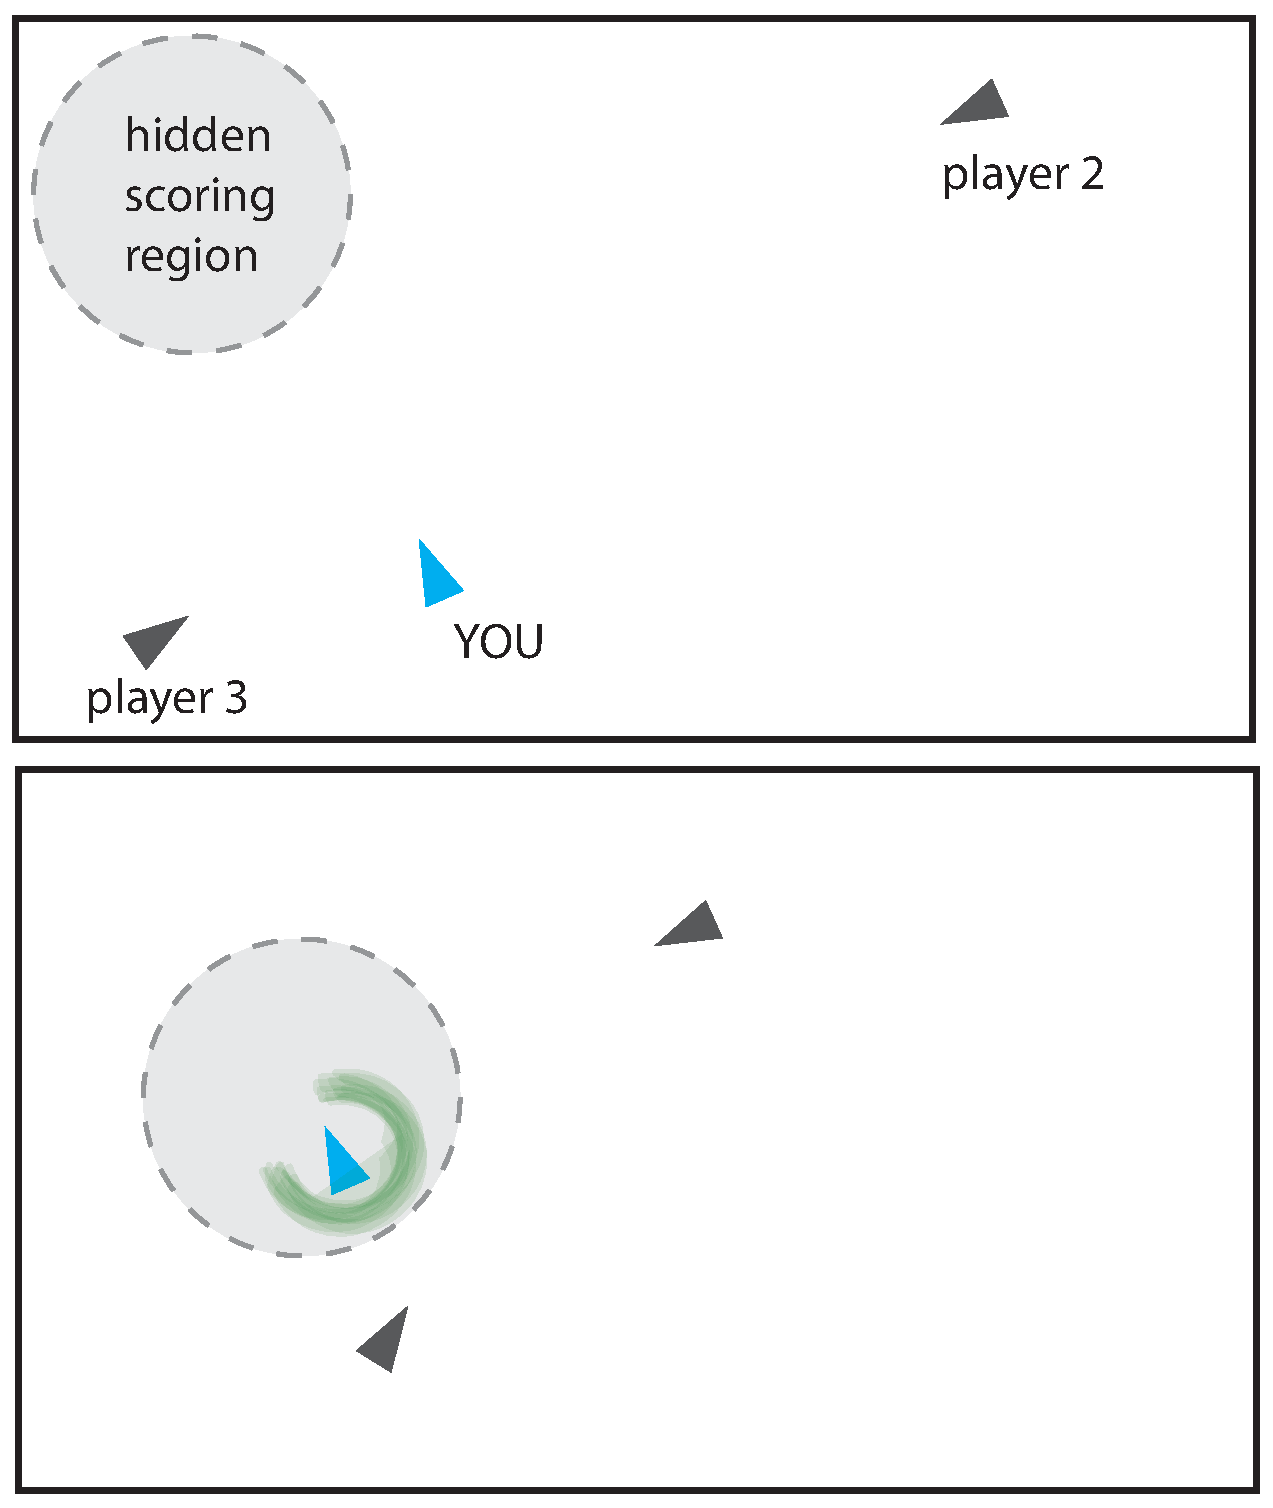
\includegraphics[width=0.6\textwidth]{./figures/experiment1_design.pdf}
  \hspace{0.1cm}
  \caption{Example states of the multi-agent tracking task used in Exp. 1. Hidden scoring region is shown in grey. Bottom frame shows participant receiving a score upon entering the region.}
  \label{fig:score}
\end{figure}

The virtual game environment measured 480 pixels in width and 285 pixels in height.
Avatars were represented by triangles that were 10 pixels in length and 5 pixels in width, rotated to the direction the avatar is facing. Players controlled their avatars by clicking and using two keyboard keys. 
Clicking within the playing area instantly oriented the direction of the avatar to be facing the location clicked. 
Participants could hold the "a" key to accelerate or hold down the "s" key to stop.  
The avatars automatically moved forward at a constant velocity of 17 pixels per second if no buttons were pressed, but instantaneously increased to a constant velocity of 57 pixels per second for the duration of time that the ``a" key was held down and decreased to 0 pixels per second for the duration of time the "s" key was held down. 

We designed the participant interface as a multi-agent tracking environment.
The score that agents obtained at each location at each point in time was determined by an underlying ``score field.'' 
This field was hidden from participants, who  only had access to the score at their current location. 
We generated score fields by first initializing a circular region with a diameter of 50 pixels at a random location on the playing area. 
Inside this region, the score was set to 1.
Outside this region, the score was set to 0.
We then moved this region along a straight line to a randomly chosen target location within the playing area at a speed of 17 pixels per second.
Once it reached this location, we selected another target location, and repeated the process for the duration of the experiment.
We pre-generated 5 such score fields, so multiple groups were randomly assigned to the same underlying field.  

Because these simple score fields were binary (i.e. either inside or outside the circular scoring region), we showed participants binary feedback about their current score.
When an avatar entered the circular region, it was surrounded by a salient sparkling star and the border of the playing area turned green. 
Critically, this feedback was only visible to the participant controlling that avatar; participants did \emph{not} directly observe whether other players were in the scoring region.

Each participant played in a single
continuous game lasting for 5 minutes, and locations were updated every 125 milliseconds. 
To discourage inactivity, participants also received 2/3 of a point for each second they were actively participating in the game.
For any moment when an avatar was touching a wall, we displayed a large warning message and set the player's current score to zero so that they stopped accumulating points.

\subsection{Procedure}

After agreeing to participate in our experiment, participants were presented with a set of instructions describing the mechanics of the game, using a cover story framing the game as a search for the "magical bonus region".  
The participants were informed about the dynamics of the underlying score field and also explicitly informed that ``There is no competition between players; the magical region is not consumed by players. It simply changes location over time." 
Participants were not explicitly instructed or suggested to cooperate or coordinate with each other.

After successfully completing a comprehension test, participants were then redirected to a waiting room.
For each waiting room we started, we randomly sampled a target group size between 1 and 6.
Participants would wait for up to 5 minutes or until the pre-assigned number of other players joined.
While in the waiting room, participants could familiarize themselves with the controls of the game.  Players were not shown any score in
the waiting room unless the participant was against a wall, in which
case the border of the playing region would turn red and a warning appeared on screen.  All players spent at least one minute in the waiting room to help ensure familiarity with the controls before starting the game. 

Both in the waiting room and the actual game, were removed for inactivity if we detected that they had switched to another browser tab for more than 30 seconds total throughout the game or if the player's avatar was unmoving against a wall for 30 consecutive seconds.  
We also removed players if their ping response latencies were greater than 125ms for more than 75 seconds in total throughout the game.  
We paid participants 75 cents for completing our instructions and comprehension checks, and the participants could receive a bonus of up to \$1.25 during the five minutes of gameplay. Each point in the game corresponded to \$0.01 of bonus. Each participant was also paid 15 cents per minute for any time spent in the waiting room, minus any time that player spent against a wall.  These numbers were chosen so that the participants were expected to receive at least a wage of \$9 per hour for the totality of their time active in the
experiment.

\todo[inline]{rdh: need to describe how we handled participant disconnects/removals (i.e. allowed the smaller group to continue)? Also, need to refer to Fig. 1 in text, and to the supplemental Fig with actual screenshots.}
We implemented this experiment using the MWERT framework \cite{hawkins_conducting_2014}, which uses a stack of recent web technologies capable of handling the challenges of real-time, multi-player web experiments, including Node.js, the Socket.io module, and HTML5 canvases.  
% Since MWERT was originally used
% for two-player games, we had to extend the MWERT framework in several
% ways to handle the challenges posed by hosting larger groups of
% players.

\begin{figure}[t!]
  \centering
  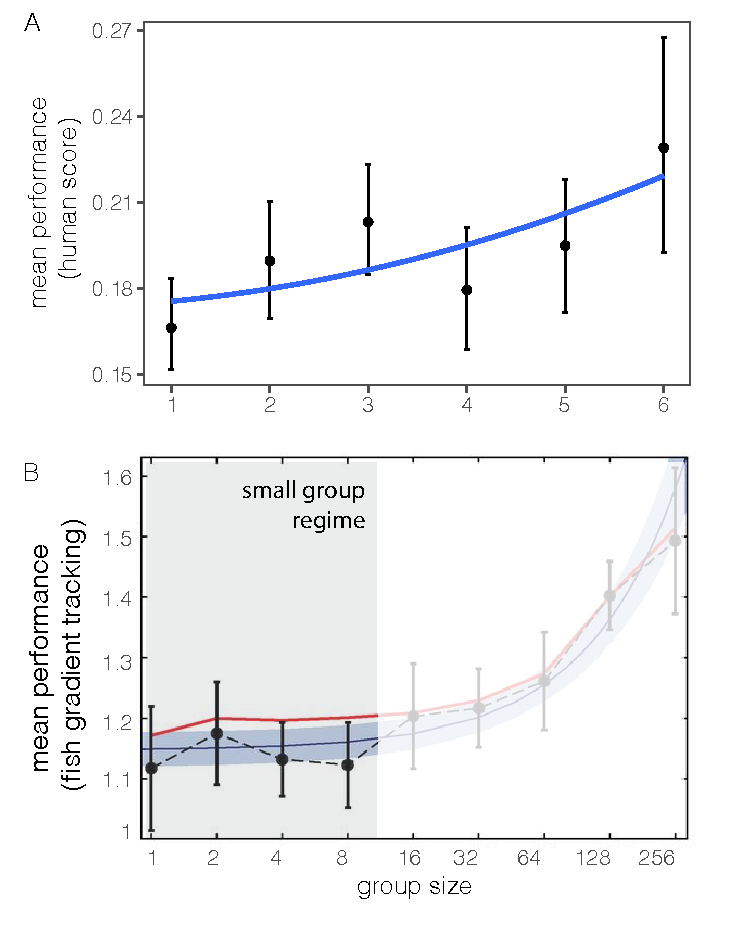
\includegraphics[width=0.8\textwidth]{./figures/exp1_combined.pdf}
  \caption{(A) Mean performance of human participants as a function of group size in Experiment 1.  Error bars are 95\% bootstrap confidence intervals using the group as the primary bootstrap unit.  All points are averages over at least two groups. (B) Mean performance of groups of fish, reproduced with permission from Berdahl et al (2013). There was no improvement in the respective small-group regime, highlighted in grey.}
  \label{fig:exp1_performance}
\end{figure}

\subsection{Results}

We hypothesized that individuals in larger groups would be able to achieve higher scores on average than individuals in smaller groups. 
To test this hypothesis, we examined performance during the second half of the 5-minute session\footnote{Results did not change when using the mean score over the entire session, but we reasoned that using the second half better controls for practice effects.}. 
We constructed a mixed-effects regression to predict each individual's score including a fixed effect of the number of other players in their environment and random intercepts for each group and each underlying score field.
We found that the performance of each individual significantly increased when they were in larger group sizes ($b = 0.91$, $t = 3.3$, $p = 0.001$; see Fig. \ref{fig:exp1_performance}A). 
This effect contrasts with the lack of improvement found by \citeA{berdahl_emergent_2013} in fish groups at the same small sizes (Fig. \ref{fig:exp1_performance}B).

\section{Experiment 2: Testing copying strategies}

What allowed humans in Experiment 1 to reap the benefits of collective intelligence at smaller group sizes than fish?
We hypothesized that human behavior in this small group regime is the consequence of two underlying strategies: (1) independent exploration and (2) precise, targeted copying based on social inferences about success. 
These strategies rely on cognitive mechanisms allowing humans to infer ``who knows'' about high-scoring locations over time based on outward behavioral traces (e.g. slowing down) and also to inhibit social influence to act independently when appropriate.
These strategies contrast with computational models explaining collective sensing in fish as an emergent consequence of two general-purpose processes: (1) the modulation of speed in preferred regions and (2) the general tendency to orient toward other agents \cite{berdahl_emergent_2013}.

For our second set of experiments, then, we designed a sequence of controlled scenarios that would be more diagnostic for testing the use of these different strategies.
We placed participants into an environment with only artificial agents, not other humans, and we manipulated the location of the score field to estimate the probability of spontaneously copying different agents under different conditions.

\subsection{Participants}

We recruited 28 unique participants from Amazon Mechanical Turk to play a single-player.
All participants were from the United
States.

\subsection{Stimuli \& Procedure}

As in our first experiment, participants were given control of an avatar to explore a virtual environment and were rewarded based on their location according to a hidden ``score field.'' 
The interface and controls were the same as in Experiment 1, but the procedure differed in several ways. 
Instead of a single 5-minute session, we designed a sequence of shorter scenarios that were informative for distinguishing between several different potential mechanisms that could be used in the game.

There were two types of initial training phases that we randomized participants across. These initial training phases corresponded to two different patterns of score field dynamics. In the first pattern, the high scoring region moved contiguously along the walls of the playing area. In the second pattern, the high scoring region moved, as in Experiment 1, from one random location to another within the playing region.  Each participant first played four one-minute long practice rounds on one of these types of score fields. In the first and third practice rounds, the score field was visible to the participant.   In the second and fourth practice rounds, the score field was invisible to the participants, as in Experiment 1.

After these four practice rounds, the participants played two more one-minute rounds that we use for data to analyze. In both of these experimental rounds, we superimposed a wall-following score field pattern and a random walk score field pattern were to create a bimodal dynamic score field. In the one of the experimental rounds, no other agents were present (non-social condition), and in the other there were four bots playing with the participant (social condition). We randomized the order of social and non-social conditions.  We included the non-social condition as a control to help us adjust our statistical analysis of behavioral mechanisms to account for behavior that looks social by chance. 

\todo[inline]{An alternative way to organize the below would be to talk about the different conditions of the environment, and then talk about what they allow us to do, instead of mushing it all together.}

Our key experimental manipulations that we used to distinguish between behavioral mechanisms people were employing in this game involved carefully controlling aspects of the score field dynamics and bot behaviors. 

\paragraph{Testing exploring behavior:} In order to better study exploring versus copying and exploiting behavior, we completely omitted the high scoring region for the first twenty of seconds or so and last twenty seconds or so of each round. During these times, all the bots were randomly exploring, with two randomly exploring all the walls (in association with the wall score field dynamic) and two exploring the entire playing region (associated with the random walk score field dynamic).  With this manipulation we are able to test if participants explored randomly or copied other players when nobody in the game was receiving a high score. 

\paragraph{Testing copying behavior:} After about ten seconds in each round, we introduced the two high scoring regions into the game, and at this time we centered one on one of the bots along the wall and the other on one of the bots exploring in the entire game region. In the non-social round, we simulated the same bots, so that the distribution of score field positions was the same across the two conditions. (The bots were not responsive to the participants behavior, only to each other.) The bot behavior was programmed according to a smart copying model. These bots explore non-socially when no bots are exploiting, and copy exploiting bots when there are any. The two bots along the wall always stayed along the wall, with any copying bot choosing to copy the wall exploiting wall bot, and the bots exploring in the entire playing region also only paid attention to each other in an analogous way. These manipulations allowed us to test whether the participant would preferentially click towards the exploiting bots, and if they had any preference for the bots who were operating on the same score field dynamics the participant had practiced on.

\paragraph{Testing exploiting behavior:} A final manipulation we conducted was to randomly in either the first half or the second half of each experimental round---just when we made the high scoring regions available---automatically grant the participant a high score no matter where they are, for roughly the ten second duration that the high scoring regions were present. The purpose of this manipulation was to see whether participants would exploit when they receive a high score, regardless of what else was going on in the environment.

\begin{table}[]
\begin{tabular}{l|l|l}
                      & Participant receiving reward & Participant not receiving reward  \\ \hline
Selectively copy  & Eagerness                  & \multicolumn{1}{l|}{Selectivity} \\ \hline
Indiscriminately copy &  \multicolumn{2}{l|}{ - Independence}  \\ \cline{1-3} 
\end{tabular}
\caption{Table of behavioral patterns we use as codes.}
\end{table}

\subsection{Results}

\todo[inline]{TODO: Double-check consistent terminology for condition names and `exploiting' through methods, results, and exp. 3}
To analyze our data from this experiment we use a mixed methods analysis involving both a qualitative coding approach and a quantitative analysis of behavioral traces and click data. 

\subsubsection{Qualitative Coding Results}

\begin{figure}[t!]
    \centering
    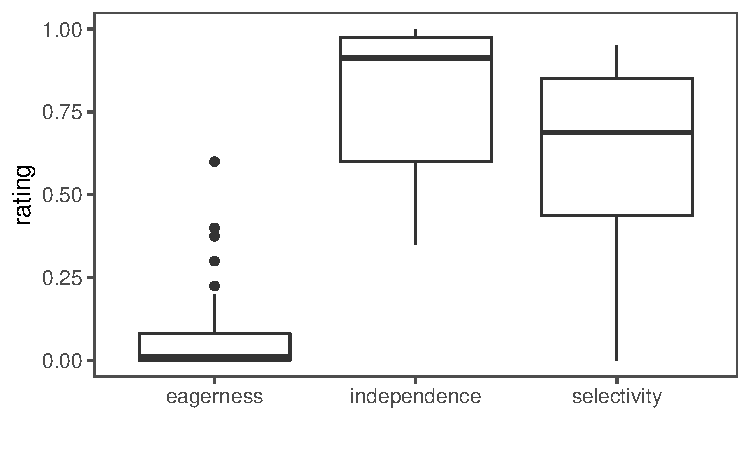
\includegraphics[width=0.9\linewidth]{figures/coding.pdf}
    \caption{Distribution of ratings for three qualitative behavioral properties that were coded from videos. Participants displayed relatively high levels of selective copying behavior and independent exploration, while eager copying is less common.}
    \label{fig:selective}
\end{figure}

For our qualitative analysis, two authors manually coded videos of our 28 participants. We coded for three behavioral signatures --- selectivity, eagerness, and independence --- on a scale from 0 to 1. \emph{Selectivity} was defined by examining behavior during the ``far'' event, when the participant was not themselves receiving a reward: selectivity was coded as an apparent preference for moving towards agents who were stopped, as opposed to moving toward agents who were moving normally or ignoring other agents.
\emph{Eagerness} was defined by  the same apparent preference for moving toward stopped agents during the ``close'' event when the participants were already receiving a high score, such that their copying behavior was not contingent on their own state.
Finally, \emph{independence} was defined by reverse-coding a general preference for moving towards agents who were \emph{not} stopped, at any point in the task\footnote{Because we never observed participants copying moving agents when they themselves were already receiving reward, this signature primarily captures whether participants were preferentially moving toward other agents during exploratory periods when there was no evidence of reward in the environment, thus we interpret low prevalence of this signature as high independence.}. 
The endpoints of the scale roughly represented the proportion of time the participant spent displaying the behavior in question compared to the potentially available opportunities to do so. 

The two authors achieved a correlation of $r = 0.75$ for selectivity, $r = 0.55$ for eagerness, and $r = 0.60$ for independence. We resolved disagreements in our codes by averaging. 
First, we found that a substantial fraction of participants display selective copying behavior and independence (Fig. \ref{fig:selective}). 
\todo[inline]{rdh: Is it appropriate to use 0.5 as a binary threshold? Do we think that midpoint is meaningful, since even lower numbers, e.g. 0.2, were indicative of some level of these signatures?}
We found that 71\% of participants had an average selectivity rating of at least 0.5, and 86\% had an average independence rating above that level. 
These proportions were significantly greater than 50\% using a two-sided binomial test, $p = 0.036$ and $p = 0.001$, respectively.  
In comparison, only 1 participant (4\%) was coded as eager at that level, which was significantly less than 50\%, $p < 0.001$.
These qualitative results show that participants appeared to selectively copy stopped agents when they themselves were not receiving reward, but otherwise mostly inhibited social influence.

\subsubsection{Quantitative Behavioral Results}

\begin{figure}
    \centering
    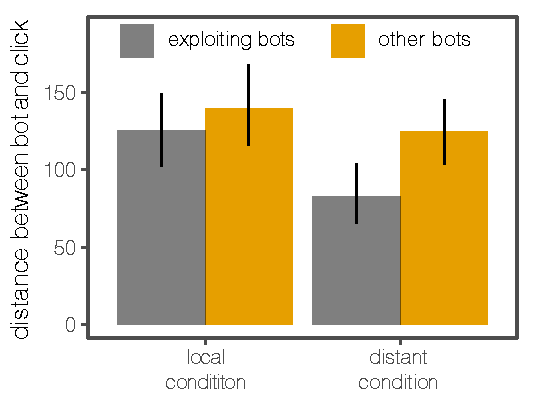
\includegraphics[width=0.8 \linewidth]{figures/proximity.pdf}
        \vspace{-1em}
    \caption{Participants selectively copy agents who are stopped but only when they themselves are not receiving reward. Error bars are bootstrapped 95\% CIs.}
    \label{fig:proximity}
\end{figure}

Next, we tested these same hypotheses quantitatively using data we recorded of participants' locations and the state of the environment at each time step of the experiment.
We operationalized copying using participant clicks.
Each click changed their avatar's destination. 
We were interested in the proximity of the new destination to other agents.
To test whether participants preferred to copy agents that displayed behavior associated with higher reward (i.e. stopping), we used information about whether each artificial agent was stopped.
To test whether participants were more likely to copy when they were not already themselves receiving a reward, we compared copying rates across the `close' condition where the score field was automatically placed on top of the participant and the `far' condition where it was only placed on top of artificial agents.
We thus constructed a mixed-effects regression model predicting the (minimum) proximity of each click to other agents as a function of condition and whether the other agents were stopped, including participant-level intercepts and main effects (the model did not converge with a random interaction term). 
We found a significant interaction, $b = 51.9, t = 4.5, p < 0.001$, showing a strong selective preference for copying other agents who appeared to be receiving reward but only in the condition when the participant was not themselves receiving a reward (see Fig. \ref{fig:proximity}). 

\section{Experiment 3: Generalizing to more complex environments}

To generalize our understanding of these mechanisms in more complex environments, and to more explicitly compare our findings to the nonhuman animal literature, we conducted a final experiment using the materials designed by \citeA{berdahl_emergent_2013} to examine collective sensing in fish.
These environments are significantly more challenging than the binary spotlight and border environments we used in Experiments 1 and 2.
They require agents to use continuous gradients to navigate noisy and fluctuating score fields.
We manipulated the level of noise across different groups, predicting that the cognitive mechanisms discussed in the previous sections would be less reliable under noisier conditions.

\subsection{Participants}
We recruited 563 unique participants from Amazon Mechanical Turk to
participate in our experiment.  All participants were from the United
States.  After excluding 72 participants due to inactivity or latency,
and 6 others for disconnecting in the first half of the game, we were
left with usable data from 437 participants in 224 groups.  These
groups ranged in size from one to six individuals.  Since we were only
able to collect one group of size six, we ignored this group in our
analysis.

\subsection{Stimuli and Procedure}

\begin{figure}
  \centering
  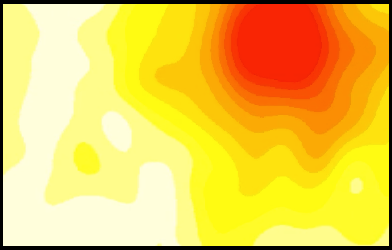
\includegraphics[width=0.4\textwidth]{./figures/easy-field}
  \hspace{0.1cm}
  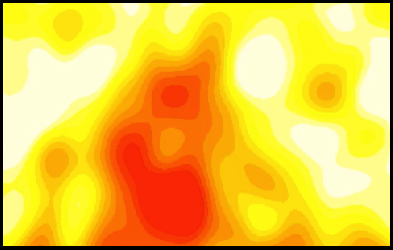
\includegraphics[width=0.4\textwidth]{./figures/medium-field}
  \caption{Example score fields from the low noise (left) and medium
    noise (right) conditions at particular points in time.  Red areas
    indicate higher scoring areas.}
  \label{fig:score_exp3}
\end{figure}


The game scores of the participants in our experiments were determined
by underlying ``score fields''.  These score fields consisted of $480
\times 285$ arrays of score values for each 125ms time interval in our
game.  We generated these score fields using the method reported by
Berdahl et al. \citeyear{berdahl_emergent_2013}. First, a
``spotlight'' of high value was created that moved in straight paths
between uniformly randomly chosen locations.  This spotlight was then
combined with a field of spatially correlated noise.  This procedure
yields a complex landscape with many transient maxima and a single
persistent time-varying global maximum.

We manipulated the weighting between the noise field and the spotlight
to generate different task conditions.  We used two weight values,
corresponding to the ``low'' and ``medium'' noise levels reported by
Berdahl et al.  Examples of score fields are shown in Figure
\ref{fig:score_exp3}.  113 individuals (63 groups) were assigned to the low
noise condition and 324 individuals (161 groups) were assigned to the
medium noise condition.  To decrease variability and increase
statistical power, we generated only four distinct score fields per
noise level, so multiple groups experienced the same fields.  To
discourage inactivity, players were awarded a score of zero,
corresponding to zero bonus, if their avatars were touching a wall.

We attempted to give our participants perceptual and motor capabilities
in this environment similar to the capabilities that Berdahl et
al. observed in the fish in their experiments.  In terms of
perception, we restricted the information that participants received
about the underlying score fields in the games.  We allowed
participants to see only the scores at their avatars' locations.  The
participants could \emph{not} see the scores that other players were
obtaining or the scores at any other locations besides their own.
However, the positions, directions, and speeds of all other players
were visible to each player.  All of this information was updated in
real-time every eighth of a second.  A screenshot of the interface we
used for the game is shown in Figure \ref{fig:exp3_interface}.
%To model the capabilities that fish were presumed by Berdahl et al. to
%have in their environment, we restricted participants to only being
%able to observe the scores at the particular locations in the game
%their avatars were occupying.  This score was displayed to the player
%at the top of the screen.  The players were also able to see their own
%positions in the environment as well as the positions, directions, and
%speeds of all other players.  This information was updated in
%real-time every eighth of a second.  Importantly, though, the
%participants could not see the scores that other players were
%obtaining.  A screenshot of the interface we used for the game is
%shown in Figure \ref{fig:interface}.

Players controlled their avatars using the left and right arrow keys
to turn (at a rate of $40^\circ$ per second) and could hold the
spacebar to accelerate.  The avatars automatically moved forward at a
constant velocity of 136 pixels per second whenever the spacebar was
not depressed.  The avatars instantaneously increased to a constant
velocity of 456 pixels per second for the duration of time that the
spacebar was held down.  We chose these speed values to match the
speeds that Berdahl et al. reported observing in their fish, and we
also matched the playing area dimensions and game duration to the
parameters of their experiments.  Each participant played in a single
continuous game lasting for 6 minutes.


After agreeing to participate in our experiment, participants were
presented with a set of instructions.  These instructions simply
described the mechanics of the game.  The participants were not
informed about the nature of the underlying score fields and were not
encouraged to work together.  After successfully completing a
comprehension test, participants were then redirected to a waiting
room.  In the waiting room participants would wait for up to 5 minutes
or until a pre-assigned number of other players joined the game.
While in the waiting room, participants could familiarize themselves
with the controls of the game.  Players were not shown any score in
the waiting room unless the participant was against a wall, in which
case the displayed score would change from a dashed line to a red
``0\%''.  We found no evidence for the amount time a player spent in
the waiting room having any effect on individual performance in the
game (linear regression slope 1.993e-06, with 95\% confidence interval
[-1e-05, 1.4e-05]).  As in the actual game, participants in the
waiting room would be removed for inactivity if the player's browser
was active in another tab for more than 15 seconds or if the player's
avatar was unmoving against a wall for 30 seconds.  We also removed
players if their ping response latencies were greater than 125ms for
more than 36 seconds.  We paid participants 50 cents for reading our
instructions, and the participants could receive a bonus of up to
\$1.25 during the six minutes of gameplay. Final bonuses were computed
to be the players' cumulative scores divided by the total length of
the game times the total possible bonus.  Following the current
convention on Mechanical Turk, each participant was also paid 12 cents
per minute for any time spent in the waiting room, minus any time that
player spent against a wall.  These numbers were chosen so that the
participants were expected to receive at least the U.S. federal minimum
wage of \$7.25 per hour for the totality of their time active in the
experiment.


\begin{figure}[t]
  \centering
  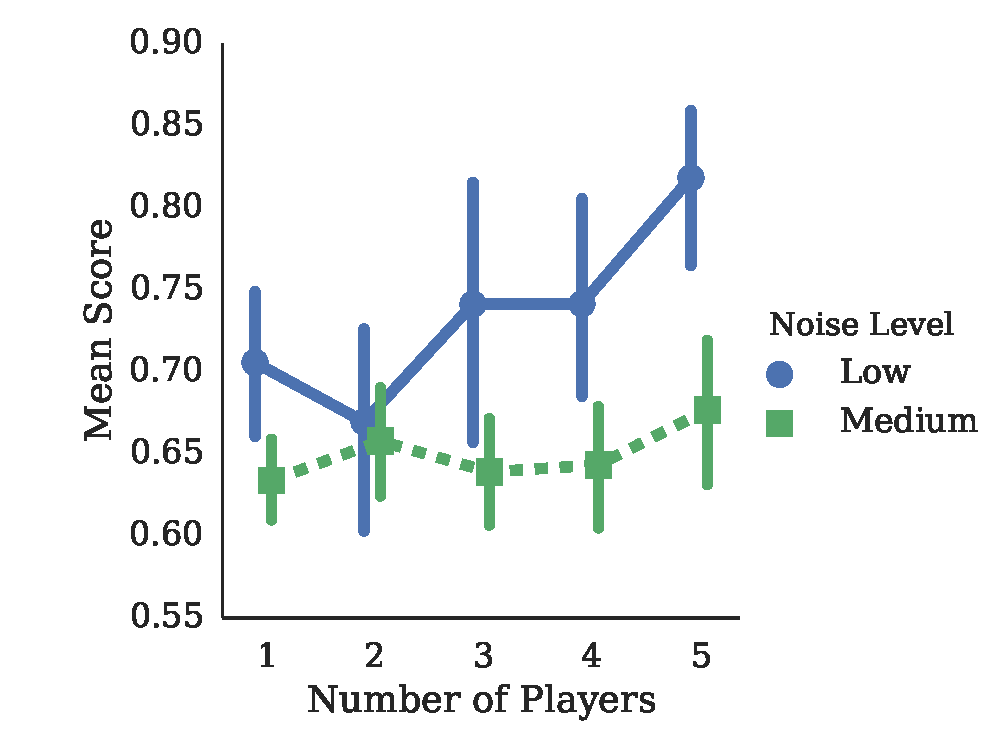
\includegraphics[width=0.4\textwidth]{./figures/performance-summary}
  \caption{Mean performance as a function of group size in the low and
    medium noise levels.  Error bars are 95\% bootstrap confidence
    intervals using the group as the primary bootstrap unit.  All
    points are averages over at least two groups.  This plot excludes
    the single group we were able to collect of size six.  Including
    this group weakens the trend in the medium noise condition.}
  \label{fig:performance}
\end{figure}

\subsection{Results}

We find that group size is positively related to group performance in
this game in the low noise condition.  However, we find that there was
little effect of group size in the medium noise condition.  Average
performance as a function of group size in each of these conditions is
shown in Figure \ref{fig:performance}.  A linear regression on the
individuals in the low noise condition produces a significant positive
slope of 0.0238 and a 95\% confidence interval (CI) of
$[0.006,0.041]$.  A linear regression on the individuals in the medium
noise condition produces a marginally significant positive slope of
$0.0068$, 95\% CI $[-0.001,0.015]$, and this trend is weakened
substantially with the inclusion of the single 6-person group.
Moreover, the marginally significant result in the medium noise
condition is driven entirely by the effect of group size in one of the
four distinct score fields we used.  This particular score field
displays a significant effect of group size with a positive slope of
0.0306, 95\% CI: $[0.015,0.046]$, while none of the others do.
Qualitative inspection revealed that this particular score field
seemed to share spatial properties more similar to the low noise score
fields, which may explain the strength of the effect in that
particular score field.  Overall these results indicate that larger
groups do tend to perform systemically better on our task than those
in smaller groups, at least in the low noise
condition.\footnote{Results were similar using a mixed-effects
  regression including group and score field as random effects, and
  also revealed larger variability due to score field in the
  ``medium'' noise condition than the ``low'' noise condition.}

In order to understand the factors that may have contributed to the
increases in performance achieved by larger groups in the low noise
condition, we examine the behavior of the players in our games.  We
assume a simple state-based representation of player behavior.  We
then attempt to identify how participants choose to occupy particular
behavioral states at each point in time, and we examine the
relationship between the players' decisions to occupy particular
states and the performance of those players.  Specifically, we assume
that at any particular point in time a player is either ``exploring'',
``exploiting'', or ``copying'' \cite<see>[for a similar
  classification]{rendell_why_2010}.  Conceptually, a player is
exploring if that player is looking for a good location to exploit, a
player is exploiting if that player has found a location where the
player wants to remain, and a player is copying if that player is
intending to move to the location of another player.

We empirically determine the state of each player at each point in
time using a set of hand-tuned filters.  All of these filters depend
only on information that is observable to any player in the game
(i.e., the filters do not depend directly on the scores of any
individuals), and hence we can use the inferred states of players as
proxies for what other players might infer as the states of those
players.  Also, since the states are not defined in terms of scores,
we can meaningfully quantify the relationship between state and
performance.

We now define the three states: exploiting, copying, and exploring.
Exploiting a particular location in the environment is not completely
trivial for players since the avatars always move at least at a slow
constant velocity.  In order to attempt to stay in a single location,
a player can either meander around a particular location or can
persistently hold down one of the arrow keys while moving at a slow
speed, which creates a tight circular motion around a particular
location.  We call this second activity ``spinning'' because of its
distinctive appearance.  We then classify a player as exploiting if
the player is spinning for 500ms or if the player moves at the slow
speed for 3 seconds and has not traveled more than two thirds of the
possible distance that the player could have traveled in that time.
The second condition is supposed to capture the meandering behavior of
individuals who have not discovered how to spin.  Copying behavior is
more difficult to identify, but appears to often be characterized by
fast directed movements towards other players.  We thus classify a
player as copying if the player is moving in a straight line at the
fast speed towards any particular other player consistently for 500ms.
We classify a player as moving towards another player if the second
player is within $60^\circ$ on either side of the first player's
straight-line trajectory.  Finally, we classify a player as exploring
if the player is neither exploiting nor copying.  Thus a player will
be classified as exploring if that player is either moving slowly but
not staying in the same general location, if the player is moving
quickly but not towards any particular person, or if the player is
moving quickly and turning.

We use these filters to analyze how players behave in our game.
First, we compute the probability of a player being in a particular
state conditional on the current score that the player is receiving.
We find that the probability of a player occupying a particular state
is closely related to that player's score.  Specifically, players in
higher scoring locations are more likely to be exploiting than
exploring or copying, but the probability that a player is exploring
or copying increases as the player's score decreases.  These results,
which are visualized in Figure \ref{fig:states}, suggest that players
are choosing their states relatively rationally.  Players will tend to
remain in good areas and will leave bad areas quickly either by
exploring independently or by copying other individuals.

\begin{figure}
  \centering
  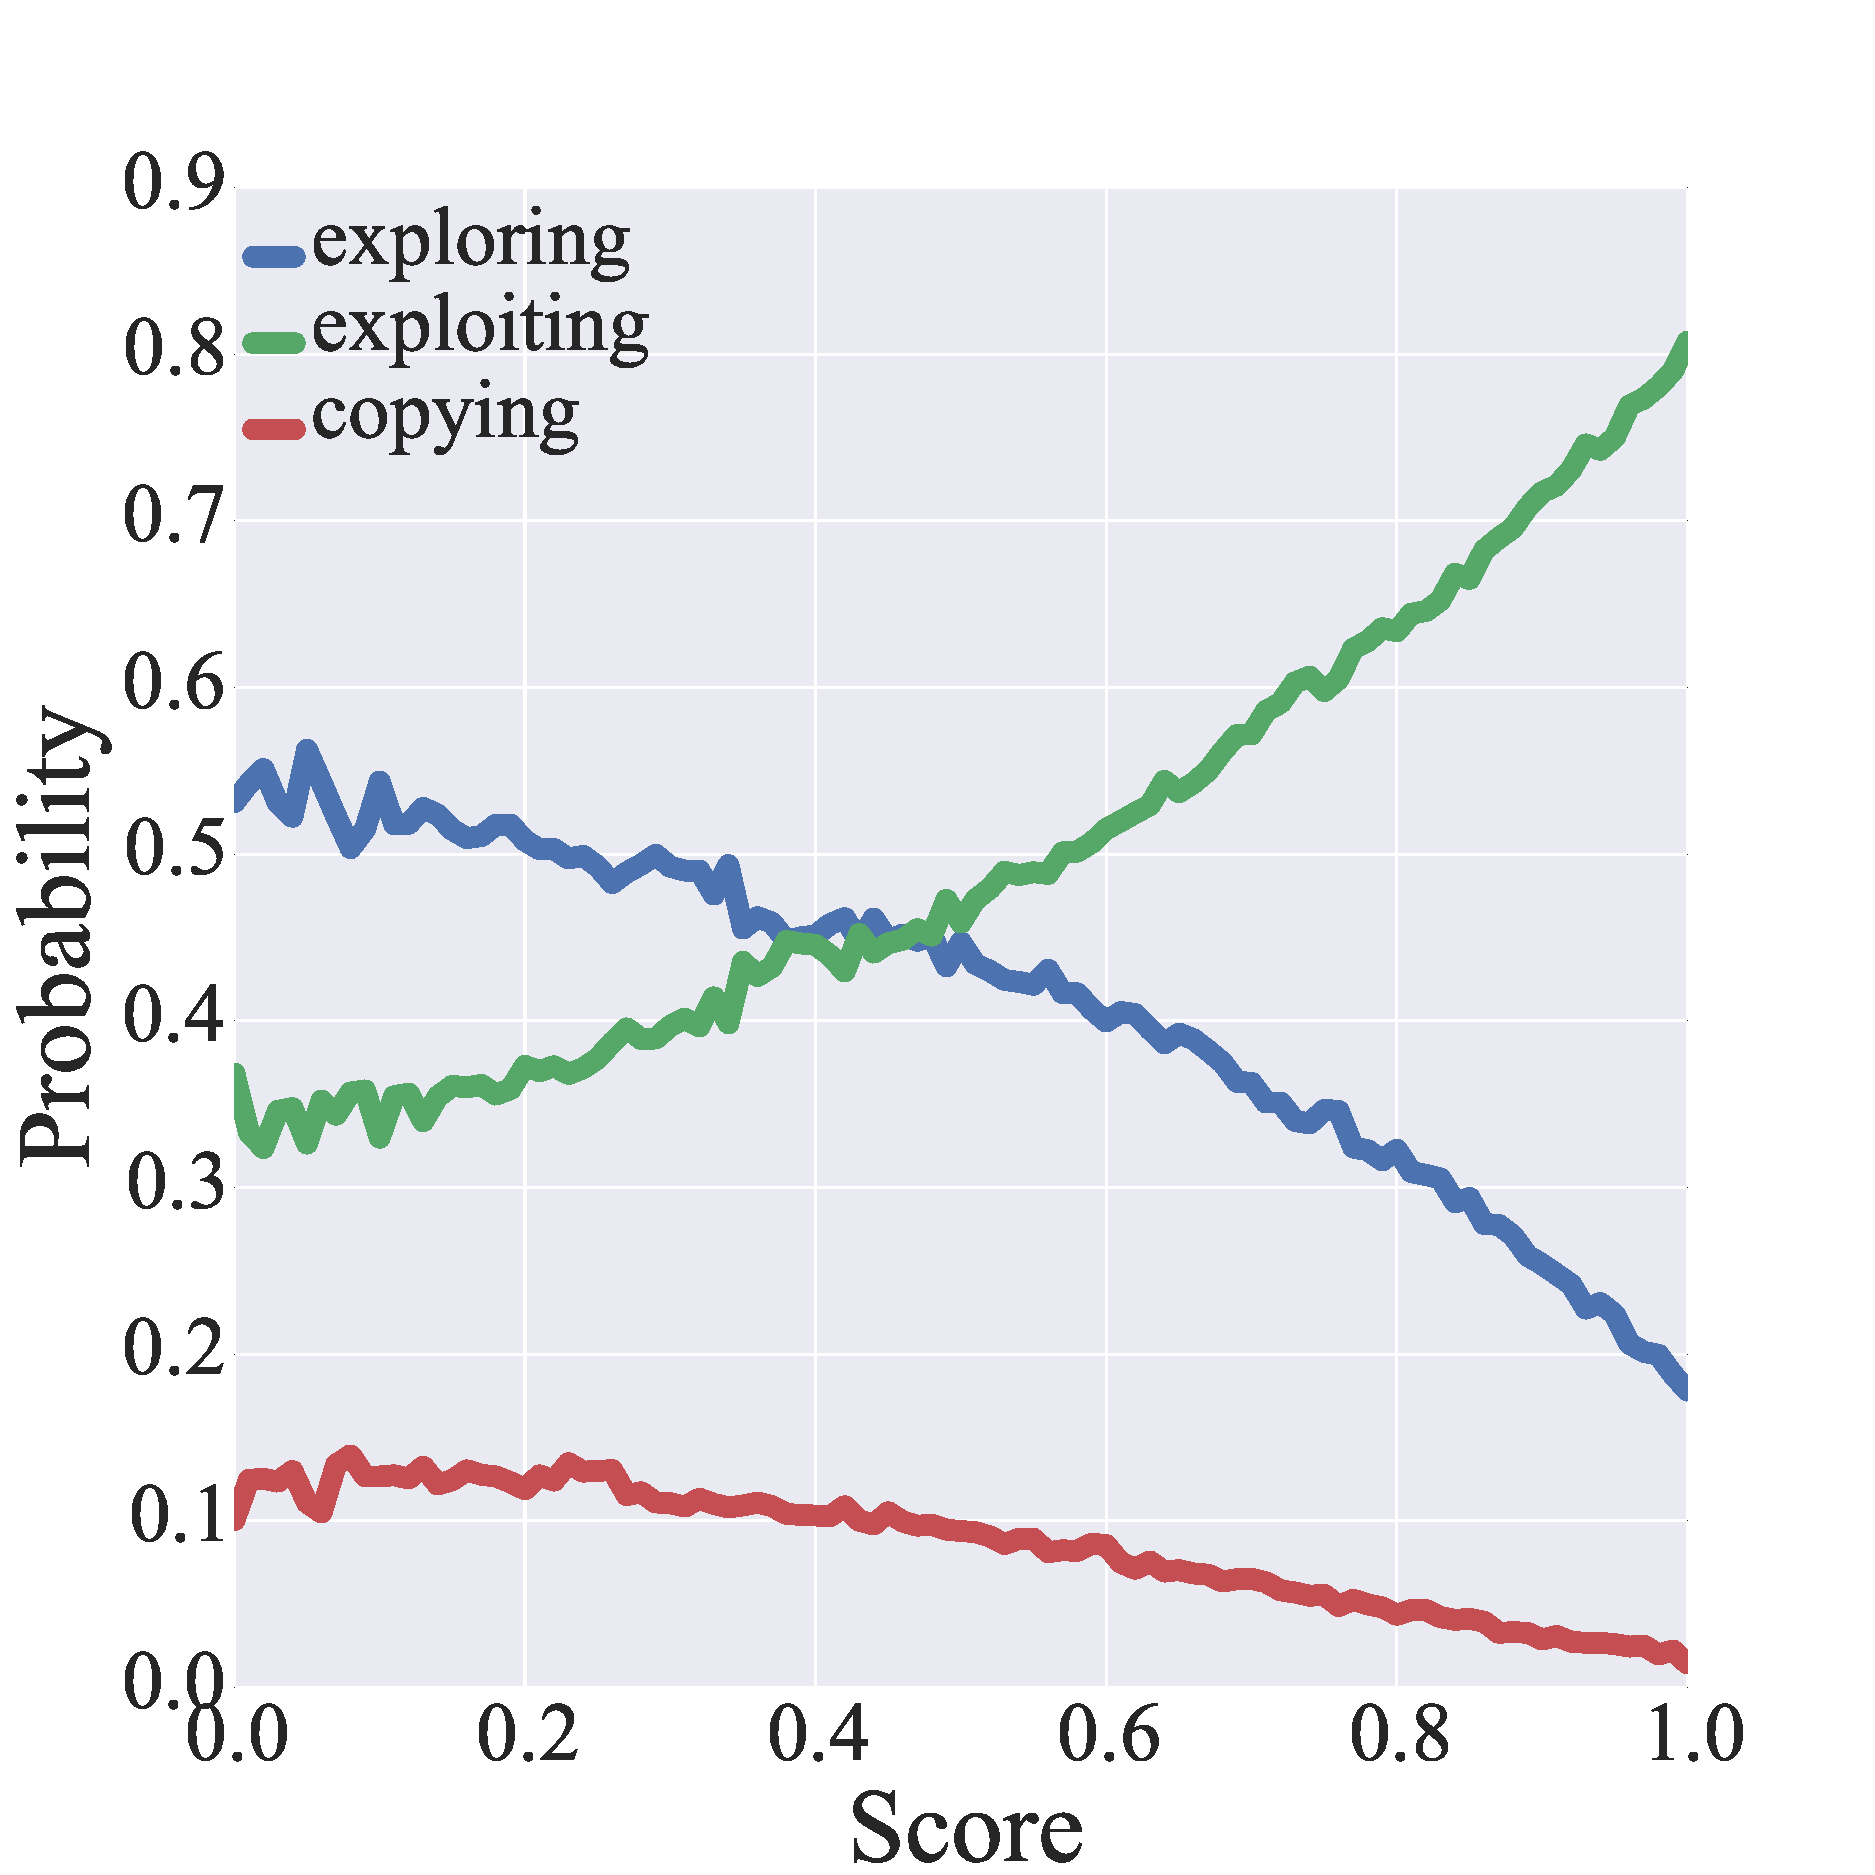
\includegraphics[width=0.29\textwidth]{./figures/states}
  \caption{The probability of an individual being in a particular
    behavioral state as a function of the individual's score.}
  \label{fig:states}
\end{figure}

Second, we find substantial variation in the types of copying behavior
that different individuals display.  Some individuals appear to focus
their copying behavior on other players who tend to have higher
scores, whereas other individuals appear to be less discriminating in
their copying behavior.  Moreover, as shown in Figure
\ref{fig:proportion}, groups that contain individuals who focus their
copying behavior on higher scoring individuals achieve significantly
higher performance in our task (slope: 0.2639, 95\% CI: $[0.145,
  0.383]$).  This result, though subject to the confounding of
correlation and causation, could be explained by theory of mind
assisting in individual and group performance.  A player who is able
to accurately infer whether another player is receiving a high score
may be able to achieve higher performance on our task by leveraging
these inferences to more effectively copy others.

\begin{figure}
  \centering
  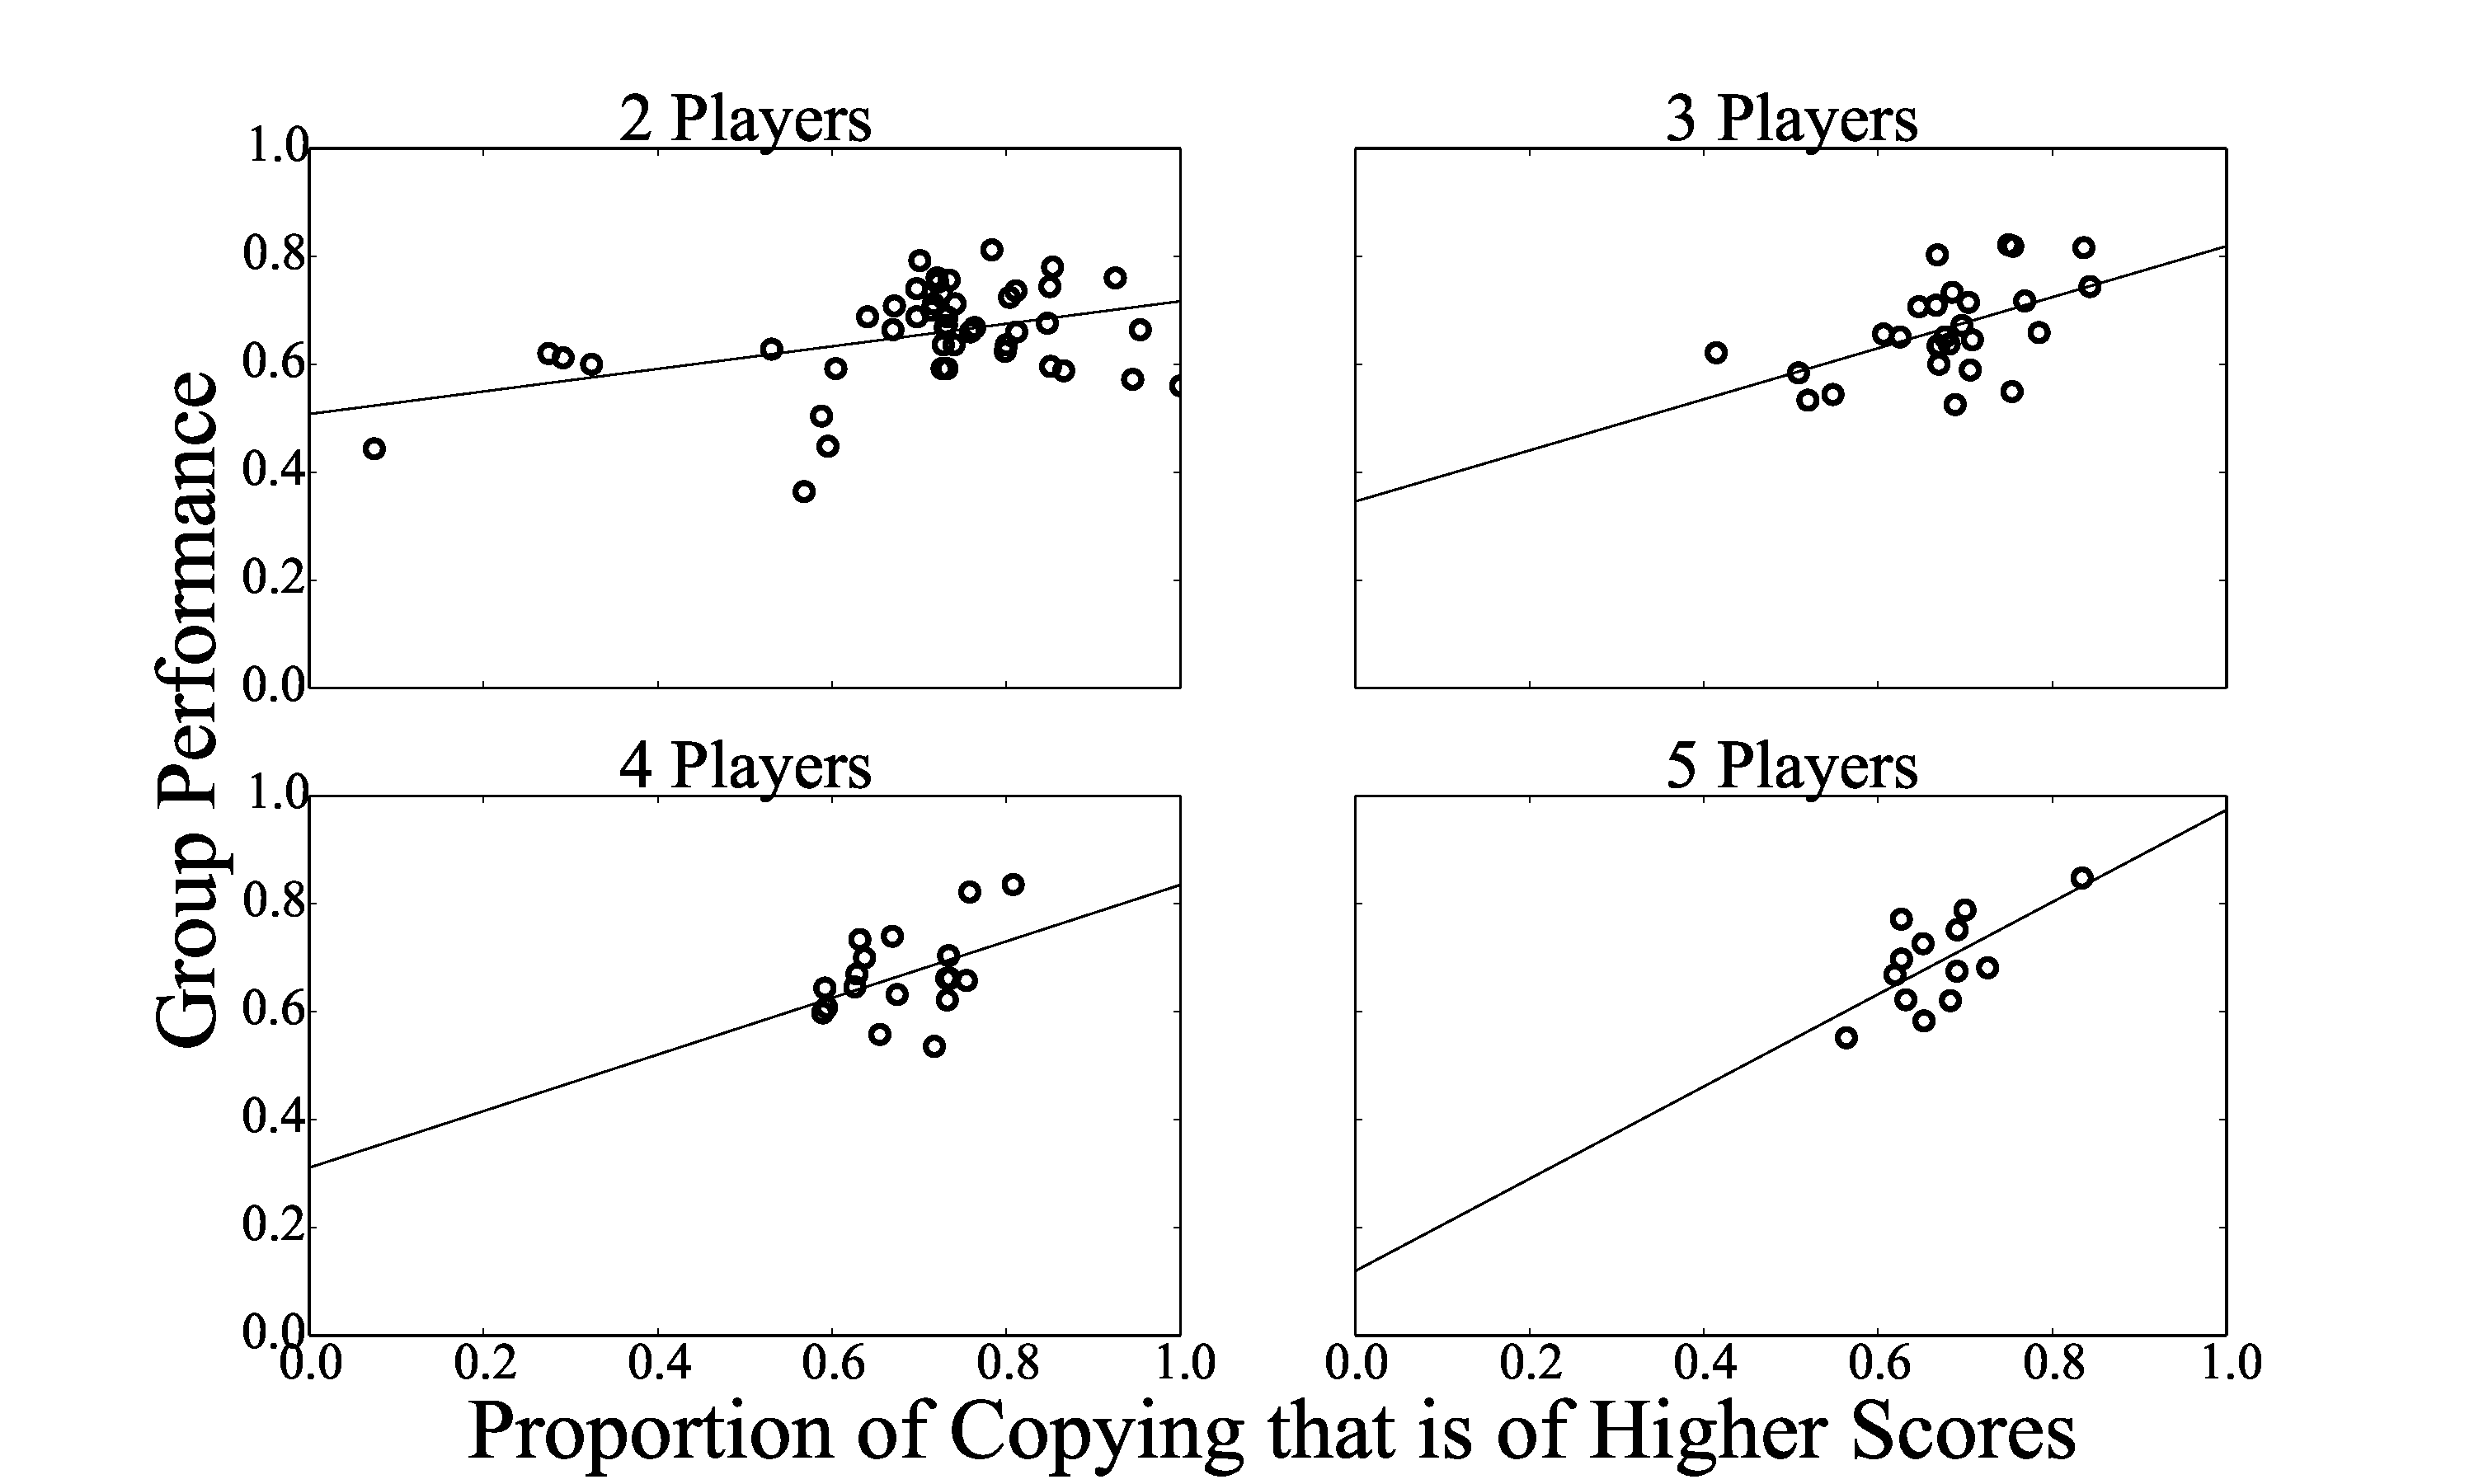
\includegraphics[width=0.5\textwidth]{./figures/copy-true-proportion}
  \caption{Average group performance as a function of the fraction of
    copying in the group that consists of ``intelligent
    copying''---copying of an individual with a higher score.  Lines
    are individually fitted regression lines.}
  \label{fig:proportion}
\end{figure}

\section{Discussion}

Our experiments established that people display collective intelligence in a multi-agent tracking paradigm inspired by experiments conducted with fish by previous researchers, and that people display emergent collective intelligence at much smaller group sizes in our environments than fish do in the setup of prior research.  In our analyses of Experiments 2 and 3, we also confirmed that agent reasoning ability underlie the way that people achieve collective intelligence in this environment.

\subsection{Group Size}

In our experiment, we observed that humans were able to achieve
increases in performance at much smaller group sizes than fish.  Fish
exhibited mild improvements in group performance at groups of 16 and
more substantial improvements at groups of 64 and 128.  However, we
see significant improvements in human performance at just five
players.  This difference may be at least partially explained by the
differences in the mechanism that humans appear to use in this task as
compared to fish.

Beyond the recent literature on collective intelligence in nonhuman
animal groups, there has been a long line of work studying the factors
that predict the performance of human groups in various scenarios
\cite{kerr_group_2004}.  Our findings are consistent with previous
work suggesting that having a larger group is beneficial in complex,
uncertain environments \cite{stewart_meta-analytic_2006}.  Unlike much
of this previous work, however, we focus here on the possibility in
larger groups of new emergent group abilities and behaviors, and on
the mechanisms leading to these emergent properties.

\subsection{Metacognitive Reasoning}

People in our experiments displayed remarkable ability to adapt to the new environment they entered for these experiments. For fish, the ability to
gain from group performance in these collective sensing tasks is
likely based on innate behaviors, selected over many generations of
fish facing exactly this problem over their whole lifespans.  In
contrast, some of our humans groups, facing this particular problem
for the first time, appear to have discovered reasonable collective
sensing strategies in just a matter of minutes.


\subsection{Agent Reasoning}

Interestingly, the mechanism we identify in humans is similar to that
of fish in some ways, but it is also distinct important ways.  Similar
to the behavior of humans in choosing appropriate states based on
current score, fish modulated their speeds based on the level of
darkness that they were experiencing.  Fish moved slower in their
preferred darker areas and faster in lighter areas.  Similar to the
copying behavior we observe, fish had a tendency for turning towards
other fish.  However, Berdahl et al.'s model of the behavior of their
fish did not require any reference to the kind of discerning social
awareness that we see in humans.  Whereas fish appear to equally
weight information from all nearby conspecifics, effective humans
appear to modulate their copying behavior based on the inferred scores
of other players. The strategic use of independent exploration (a form
of asocial learning) was also key to the mechanism enabling human
success. These key differences support recent work in social learning
\cite{wisdom_social_2013, mcelreath_beyond_2008}, which find an
impressive flexibility in the strategic deployment of imitation in
humans. 

\subsection{Limitations}

Of course, it is difficult to compare human performance
directly to that of fish given the differences between the perceptual
and motor abilities of fish in an actual fish tank and the abilities
of the participants in our simulated environment.  


%Nevertheless, our comparison hints at a superior capacity for distributed cognition in humans, possibly enabled by our ability for theory of mind.

\subsection{Contextual Factors}

The picture of collective intelligence in humans and across specifies that is emerging from the scientific literature is that different mechanisms give rise to collective intelligence in different species, and that certainly the same can be said even of the different types of human collective intelligence displayed in different contexts.  Human collective intelligence on Wikipedia operates in a way that is very different from human collective intelligence (or unintelligence) on social media platforms like Twitter, and both are quite different from the mechanisms of collective intelligence through which bees find new homes or ants scavenge for food. 

The mechanisms we identify in our experiment are yet another context.

Still, the quest continues for what general abilities and principles underlie the range of intricate and sophisticated forms of human collective intelligence, and distinguish those as a group from the apparently simpler, more swarm-like forms of collective intelligence found in species such as social insects or fish.  Focusing on abilities rather than mechanisms potentially provides a slightly more domain-general way to understand collective intelligence.

\section{Conclusion}

Our work sheds light on one of the pressing puzzles of
human collective intelligence and human distributed cognition.  What
are the abilities that underlie specific mechanisms by which humans establish effective
coordinated distributed information processing agents that can
accomplish more than any individual alone?  The perspective of group behavior as
distributed processing \cite{hutchins_cognition_1995} suggests the
importance of communication for collective intelligence because of the
importance of communication in distributed systems.  Moreover, theory
of mind---an enabler of implicit communication---has been shown to be
predictive of collective intelligence \cite{woolley_evidence_2010,
  engel_reading_2014}.  Our work further
suggests that one of the roles that theory of mind plays in the
emergence of collective intelligence is facilitating implicit
communication that allows for coordination on good collective actions.
Moreover, our work also suggests that the benefit of a group's
coordinating on good actions could be more than simply the benefit to
each individual independently.  By combining a natural human tendency
for independent exploration with a discerning social awareness, humans
appear to be able to fluctuate between exploiting known good actions,
independently exploring new options, and intelligently copying the
promising choices of other individuals.  A simultaneous combination of
these activities by a cohesive group appears to lead to a collective
memory of recently good actions from individuals who continue to
exploit, and a collective movement towards actions that promise to be
good in the near future driven by independently exploring individuals.
The reactive distributed sensing ability that appears to emerge from
this process may confer a unique benefit to working together in
tightly knit groups.
%%who either find new good areas or return to the group.
%% The exploiting
%% core form the body of the group and the exploring individuals form the
%% sticky appendages that drive the group's gradual crawl.

\section{Acknowledgments}

\small

This material is based upon work supported by the National Science
Foundation Graduate Research Fellowship under Grant No. 1122374 to PK
and Grant No. DGE-114747 to RXDH. Any opinion, findings, and
conclusions or recommendations expressed in this material are those of
the authors(s) and do not necessarily reflect the views of the
National Science Foundation.  This material is based upon work
supported by the Center for Minds, Brains and Machines (CBMM), funded
by NSF STC award CCF-1231216.


\bibliographystyle{apacite}

\setlength{\bibleftmargin}{.125in}
\setlength{\bibindent}{-\bibleftmargin}

\small{
  \bibliography{couzin}
}


\section*{Appendix A: Behavioral Model}

The trends we observe suggest a potential set of behavioral mechanisms
that effective human groups may use in our task.  We propose that each
player in an effective group chooses a state based on the following
rules:
\begin{enumerate}
\item
  If the player is in a good area, the player will remain in that area
  exploiting.
\item
  If the player in not in a good area and the player perceives another
  person as possibly having a higher score, the player may choose to
  copy that person.
\item
  Otherwise the player will explore independently.
\end{enumerate}

According to this model, players in bad locations improve their scores
by copying exploiting individuals instead of wasting time by copying
low scoring players or wasting time by exploring many poor quality
areas.  The model also has interesting emergent collective properties.
When any individual finds a good area, that player will attract the
other players to that location by exploiting.  Then, when all the
players are together in a group exploiting a particular area, one of
the players will start to lose bonus as the score field shifts.  This
player will then either move closer to the others who are still
exploiting or will shift to an exploring state.  If that player starts
exploring but doesn't find any good locations, the player will return
to the group if the group is still exploiting.  If that player does
find a new good area, though, the player will start exploiting that
area.  The rest of the group will then follow after the highest
scoring region shifts to where the exploiting player is.  This
mechanism creates a kind of gradual crawling that effectively tracks
the moving score field.  Thus, by using this mechanism players are
improving both their own performances directly and also that of the
entire group by participating in this process of emergent collective
sensing.  An example of this process occurring in participant gameplay
is shown in Figure \ref{fig:example}.

\begin{figure*}
  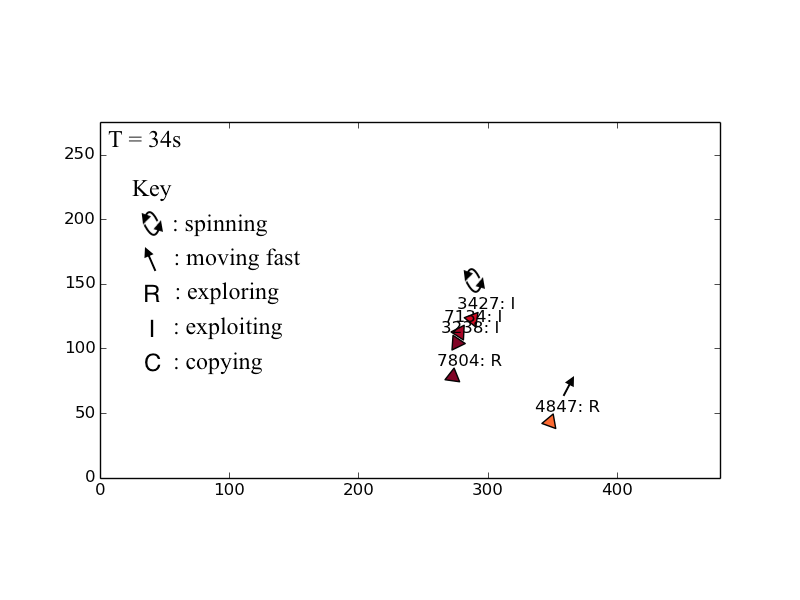
\includegraphics[width=0.33\textwidth,trim=2.5cm 3cm 2cm 3cm,clip]{./figures/pos0274}
  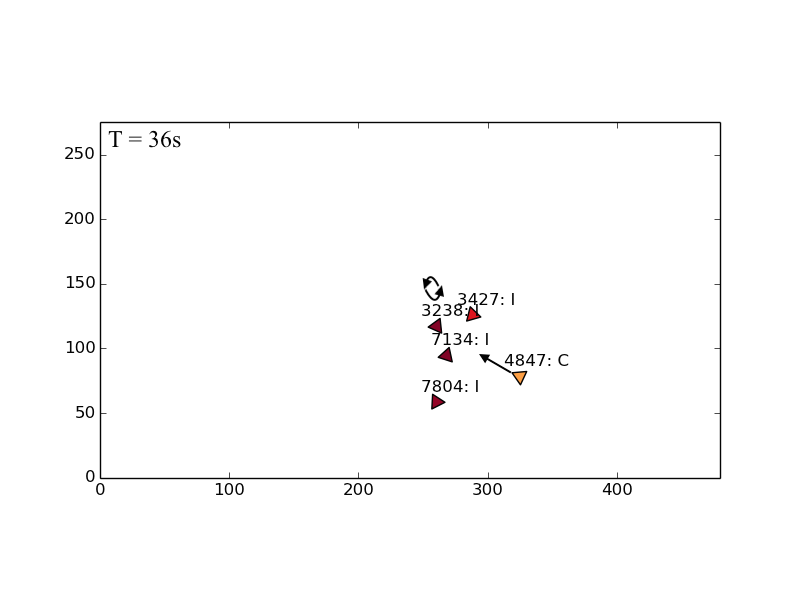
\includegraphics[width=0.33\textwidth,trim=2.5cm 3cm 2cm 3cm,clip]{./figures/pos0285}
  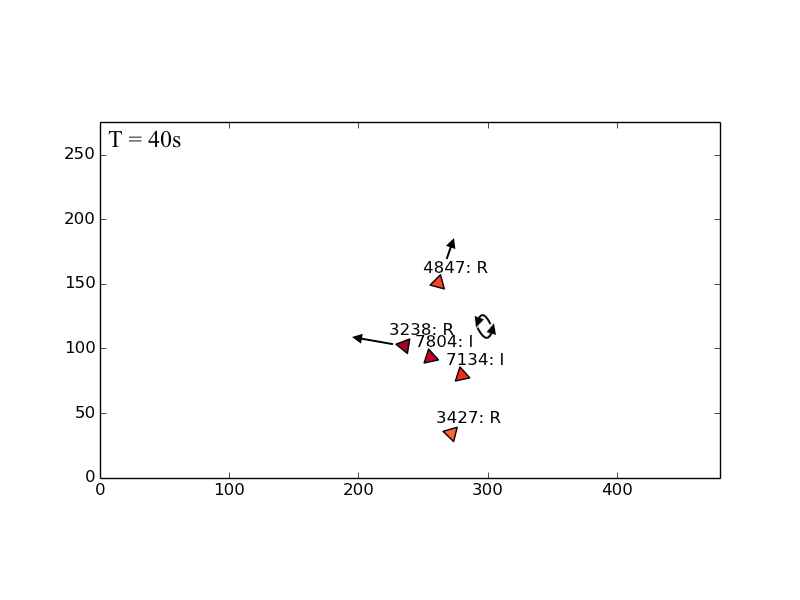
\includegraphics[width=0.33\textwidth,trim=2.5cm 3cm 2cm 3cm,clip]{./figures/pos0323}\\
  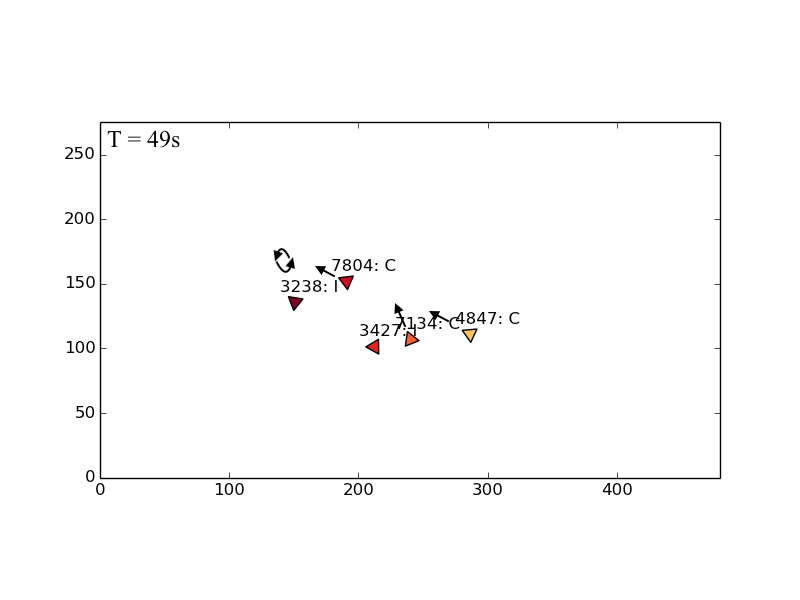
\includegraphics[width=0.33\textwidth,trim=2.5cm 3cm 2cm 3cm,clip]{./figures/pos0394} % 388
  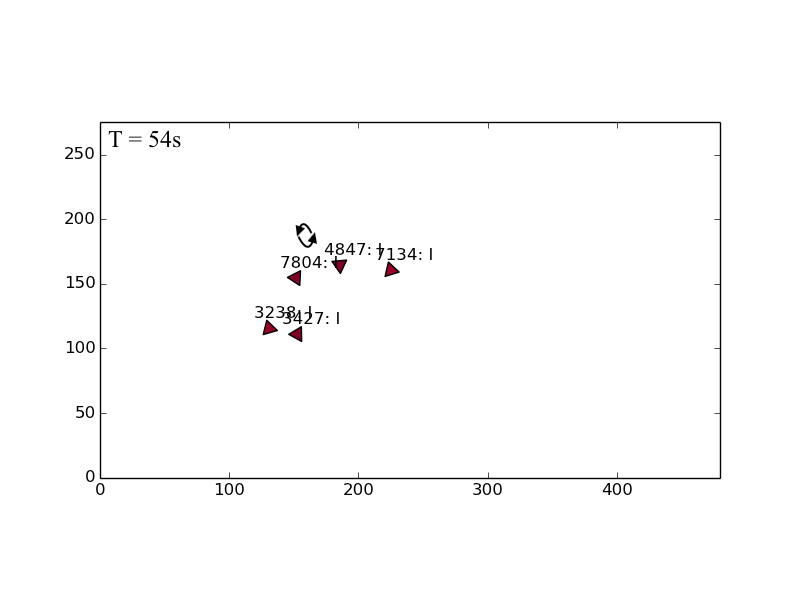
\includegraphics[width=0.33\textwidth,trim=2.5cm 3cm 2cm 3cm,clip]{./figures/pos0435}
  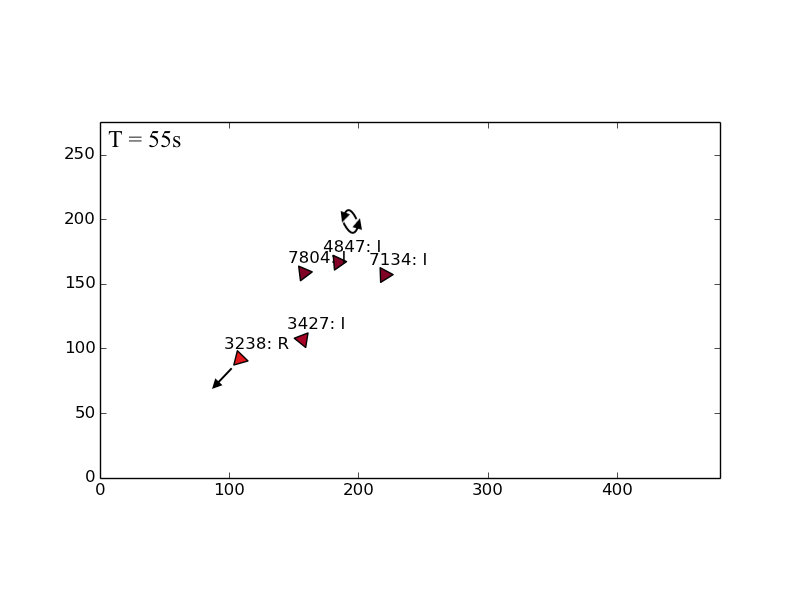
\includegraphics[width=0.33\textwidth,trim=2.5cm 3cm 2cm 3cm,clip]{./figures/pos0441}
  \caption{Reconstructions of actual gameplay in a five-person group
    illustrating both failed exploration leading to intelligent
    copying and successful exploration leading to collective
    movement. Colors indicate the individuals' scores, with red being
    higher and orange/yellow being lower.  The player labels indicate
    both player IDs and also the player states our feature extraction
    procedure inferred.  Other annotations are provided to give a
    sense for the game dynamics.  At $34$ seconds, in the first panel,
    most of the group has converged on exploiting a particular area
    while one individual is exploring independently.  To the right, at
    36 seconds, the exploring individual appears to have failed to
    find a good location and ceases exploring by copying the group.
    At 40 seconds, the final panel in the first row, the score field
    has shifted and some of the group begins exploring while others
    continue to exploit.  By 49 seconds, the first panel in the second
    row, one of the exploring individuals found a good location, and
    other players have begun to move towards that individual.  At 54
    seconds, the entire group is exploiting the new area.  In the
    final panel, at 55 seconds, the background has shifted enough
    again that one of the individuals begins to explore.}
  \label{fig:example}
\end{figure*}


\begin{figure}
  \centering
  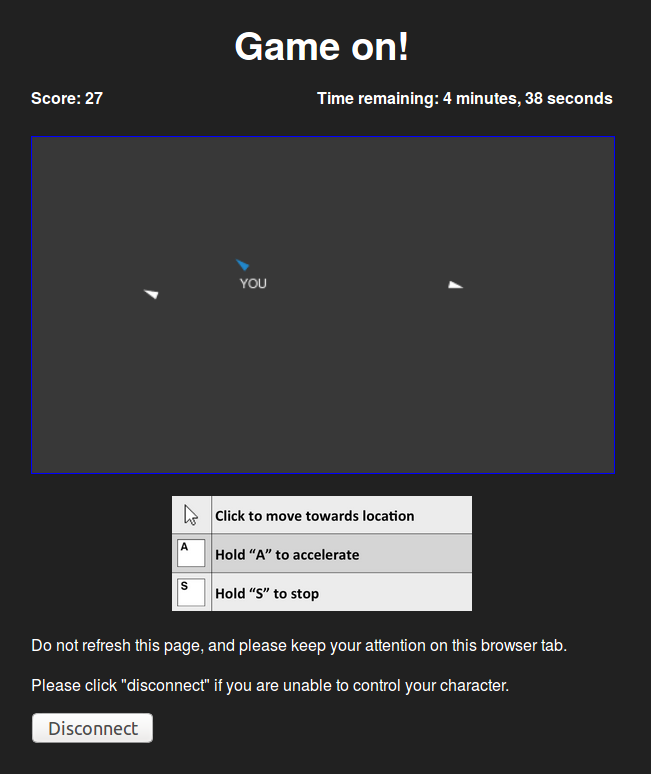
\includegraphics[width=0.3\textwidth]{./figures/experiment-3-no-score}
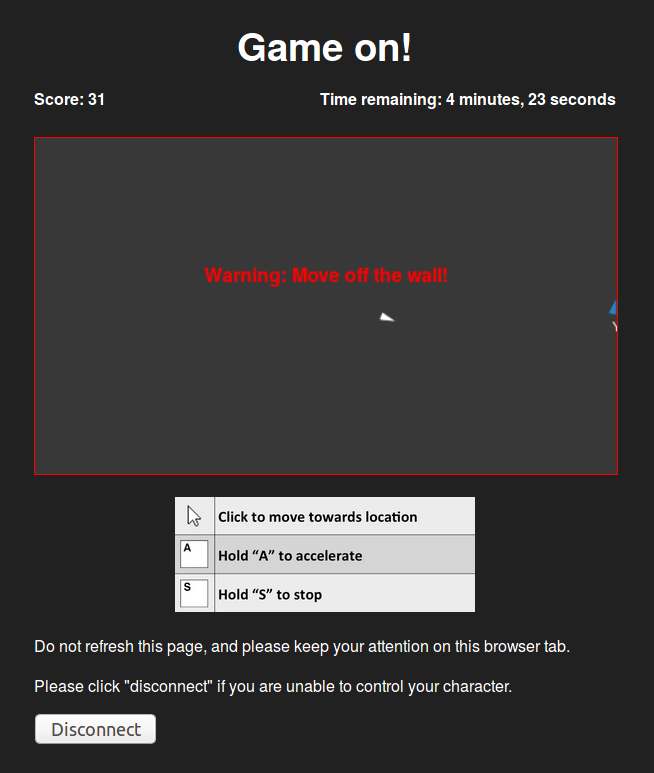
\includegraphics[width=0.3\textwidth]{./figures/experiment-3-wall}
  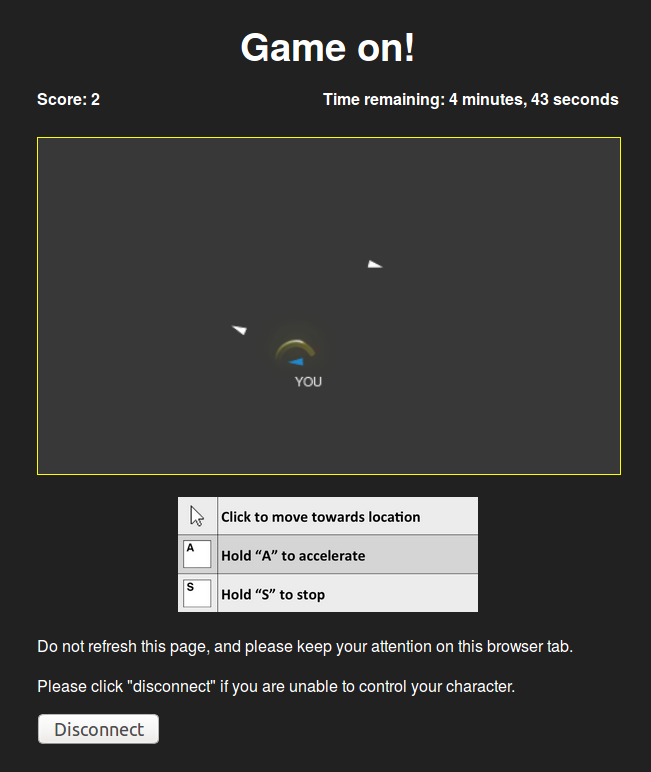
\includegraphics[width=0.3\textwidth]{./figures/experiment-3-score}
  \hspace{0.1cm}
  \caption{Examples of Experiment 1 interface.}
  \label{fig:supplemental_interface}
\end{figure}


\begin{figure}
  \centering
  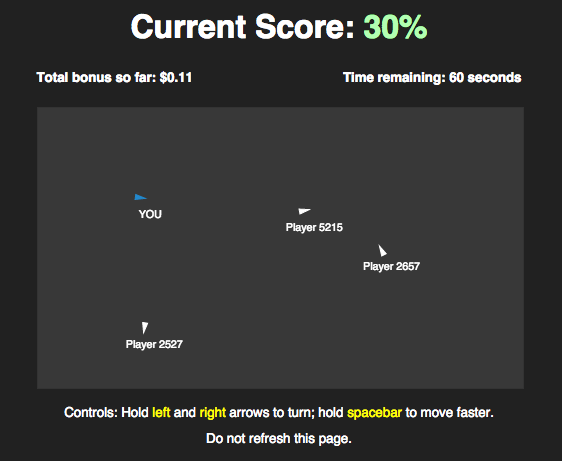
\includegraphics[width=0.9\textwidth]{./figures/interface}
  \caption{Screenshots of the Experiment 3 interface.  The
    score displayed corresponds to the value of the score field at the
    location that the player's avatar is occupying.}
  \label{fig:exp3_interface}
\end{figure}

\end{document}
